\chapter{Ambiente Universitário}

\begin{center}
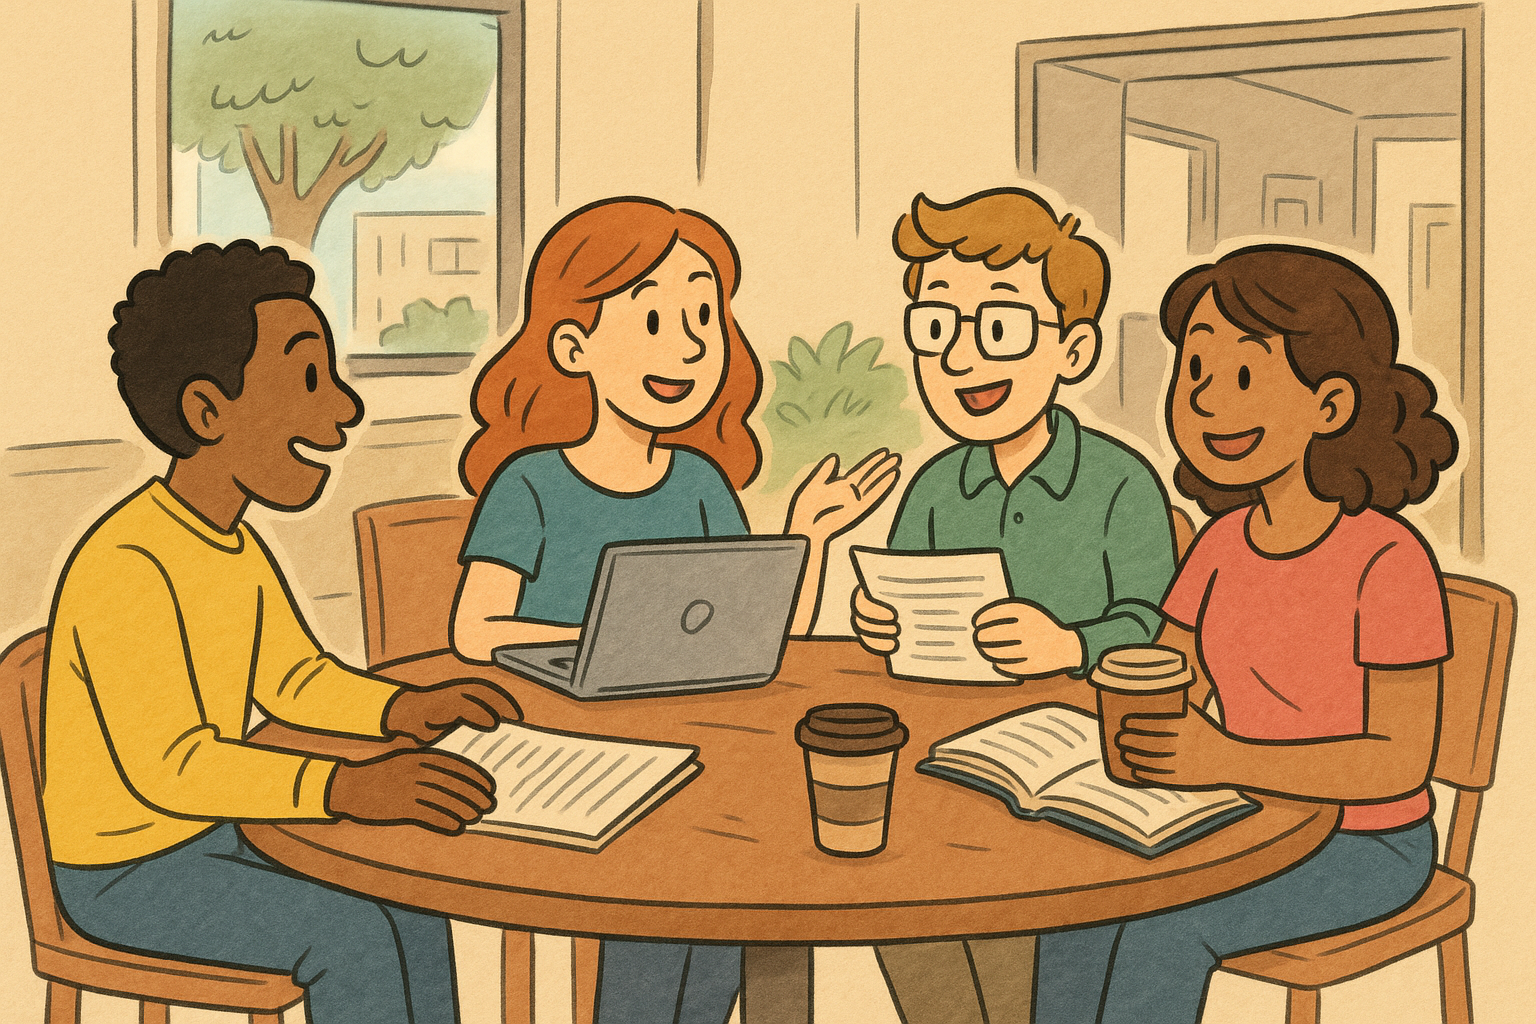
\includegraphics[width=0.5\linewidth]{Images/ambiente.png}    
\end{center}
\vspace{0.5cm}

A vida acadêmica não se faz apenas diante do computador, nem se resume às leituras solitárias em casa. A universidade é um espaço de convivência, troca de ideias e amadurecimento intelectual coletivo. Frequentar o ambiente universitário é essencial para o desenvolvimento como pesquisador.

\gxatencao{Vá ao campus. Vá ao laboratório. \\ Participe da vida acadêmica.}

É no cotidiano da universidade que os vínculos se constroem: o café no intervalo da manhã pode render uma dica de artigo importante; uma conversa no corredor pode virar uma parceria de publicação; um almoço pode trazer \textit{insights} sobre como lidar com a banca ou conseguir bolsas. 

Evitar o isolamento é uma escolha estratégica. Trabalhar exclusivamente de casa, sem interação direta com colegas ou com o orientador, reduz enormemente suas oportunidades de aprendizado informal e de inserção no ambiente científico. O pós-graduando que se isola perde acesso a uma rede viva de apoio intelectual, emocional e prático.

A socialização acadêmica — por mais informal que pareça — é um dos principais mecanismos de aprendizado e inserção na comunidade científica. Para isso: 

\begin{itemize}
    \item Frequente os seminários do seu grupo de pesquisa e os da pós-graduação como um todo.
    \item Participe de eventos promovidos pelo seu orientador, como bancas, reuniões abertas, defesas e seminários.
    \item Vá às defesas dos seus colegas, especialmente aqueles da sua turma. Isso ajuda a entender o formato, a postura esperada, o estilo das perguntas — e você pode ser lembrado por esses colegas no futuro.
    \item Quando souber quem será sua banca, procure assistir a defesas em que esses professores participem. Isso ajuda a entender o estilo de cada um e o nível de exigência esperado.
\end{itemize}

\section{Troca entre colegas}

Mantenha diálogo constante com seus colegas de laboratório, de disciplina e de pesquisa. Muitos caminhos que parecem difíceis para você já foram percorridos por alguém da sua turma. E, da mesma forma, você pode oferecer contribuições valiosas para os outros. A pesquisa é um processo coletivo, ainda que cada tese seja individual.

Não se torne um ``capacitor'' de informações. aquele que acumula tudo para si e não compartilha nada. O pesquisador que guarda o conhecimento como vantagem competitiva mina a própria reputação e prejudica o avanço coletivo do grupo.

Ao contrário, o bom pesquisador é aquele que aprende, compartilha, escuta, ensina e cresce junto. Esse é o espírito de um ambiente universitário saudável, maduro e produtivo.

A universidade é muito mais do que um local físico — é uma cultura, uma rede, um fluxo contínuo de interações. Aproveite isso. Construa pontes. Seja presente. A tese é sua, mas o caminho não precisa ser solitário.
